\documentclass{report}
\usepackage{geometry} % Page layout
\usepackage{multicol,caption} % Multiple columns
\usepackage{fancyhdr}
\usepackage{titlesec} % Section formatting
\usepackage{setspace} % Setting line spacing
\usepackage[backend=biber,style=apa,citestyle=authoryear]{biblatex}

\usepackage{lipsum} % dummy text

\renewcommand*{\nameyeardelim}{\addcomma\space}
\DeclareDelimFormat[parencite]{finalnamedelim}{\addspace\&\space}
\addbibresource{references.bib}

\newenvironment{minifig}
  {\noindent\minipage{\linewidth}}
  {\endminipage}

\geometry{landscape, margin=0.5in}
\setlength{\columnsep}{1cm}
\setlength{\columnseprule}{0.5pt}
\pagenumbering{gobble}

\pagestyle{fancy}
\lhead{Jayden Lefebvre}
\rhead{SAFS3530 Trent University}
\setlength{\headheight}{36pt}

\titleformat{\section}{\normalfont\fontsize{12}{15}\bfseries}{\thesection}{1em}{}

\begin{document}

\begin{center}
  \LARGE
  Ethylene Exposure and Shoot Growth in Early Vegetation of \textit{Narcissus sp.}
\end{center}

\medskip

\begin{multicols}{3}

  \textbf{Abstract}\\
  The effect of different concentrations of ethylene (C\textsubscript{2}H\textsubscript{4}) gas on plant bulb phenology is investigated.
  Apples are used as a source of ethylene gas in a closed greenhouse system, and bulb shoot height is measured over a period of five weeks.
  Final leaf height is plotted against with ethylene concentration, and leaf growth and growth rate are compared between control and ethylene-treated groups.
  Results were largely inconclusive, indicating poor experimental design or the influence of outside factors.
  
  \textbf{Introduction}\\
  Ethylene is a plant growth regulator responsible for fruit ripening and cell senescence.
  It has been reported in literature that exposure to ethylene can negatively impact plant shoot elongation in bulbous plants \parencite{bulbous}, and even induces leaf abscission (i.e. death) after long periods of exposure \parencite{abscission}.
  Literature findings indicate that the mechanism underlying these phenomena relate to the inhibition of auxin synthesis or enhancing auxin destruction \parencite{senescence}.
  The purpose of this study is to investigate the effect of ethylene exposure on the growth and growth rate of early vegetation in \textit{Narcissus sp.} bulbs.
  It is predicted that, due to the effect on auxin metabolism, ethylene exposure will inhibit shoot elongation in the early stages of plant growth.
  It is thus hypothesized that greater ethylene exposure will negatively influence leaf height in plant bulb vegetation.

  \vfill\null
  \columnbreak
  
  \textbf{Methods}\\
  % Each apparatus will have 1: pot (with soil and bulb), apple (excluding the control), skewer, cover and 2-4 elastic bands. The set-up apparatus will be a closed system that will contain the ethylene given off by the apple. Each plant pot and bulb is under one cover acting as a mini-greenhouse.
  Twenty-four (24) bulbs of \textit{Narcissus sp.} are planted individually in pots with organic nutrient-rich soil.
  Each pot is covered with a plastic cover, and an organic washed apple is placed inside the cover.
  The covered pot acts as a closed system to contain the ethylene given off by the apple.
  Ethylene concentration is measured at day 7.
  Leaf height is measured using calipers on a (bi-)weekly basis for five weeks.

  \textbf{Results}\\
  Below are two graphs: Figure 1 shows the \textit{final} (day 35) leaf height vs ethylene concentration at day 7, with linear regression and coefficient of determination; Figure 2 shows the average leaf height over time per ethylene treatment \textit{group} (\textbf{Control}, \textbf{High} ethylene, and \textbf{Low} ethylene), each with linear regression.

  \begin{minifig}
    \centering
    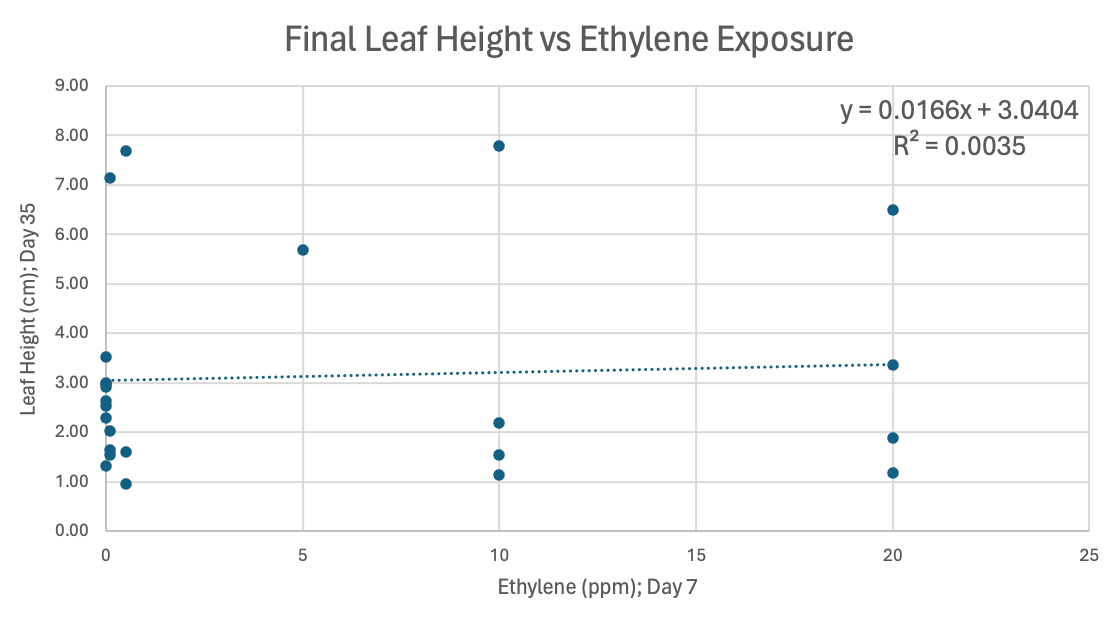
\includegraphics[width=\linewidth]{graph2.png}
    \captionof{figure}{Final (Day 35) leaf height vs ethylene concentration (Day 7) in \textit{Narcissus spp.} vegetation.}
    \medskip
  \end{minifig}
  \vfill\null
  \columnbreak
  \begin{minifig}
    \medskip
    \centering
    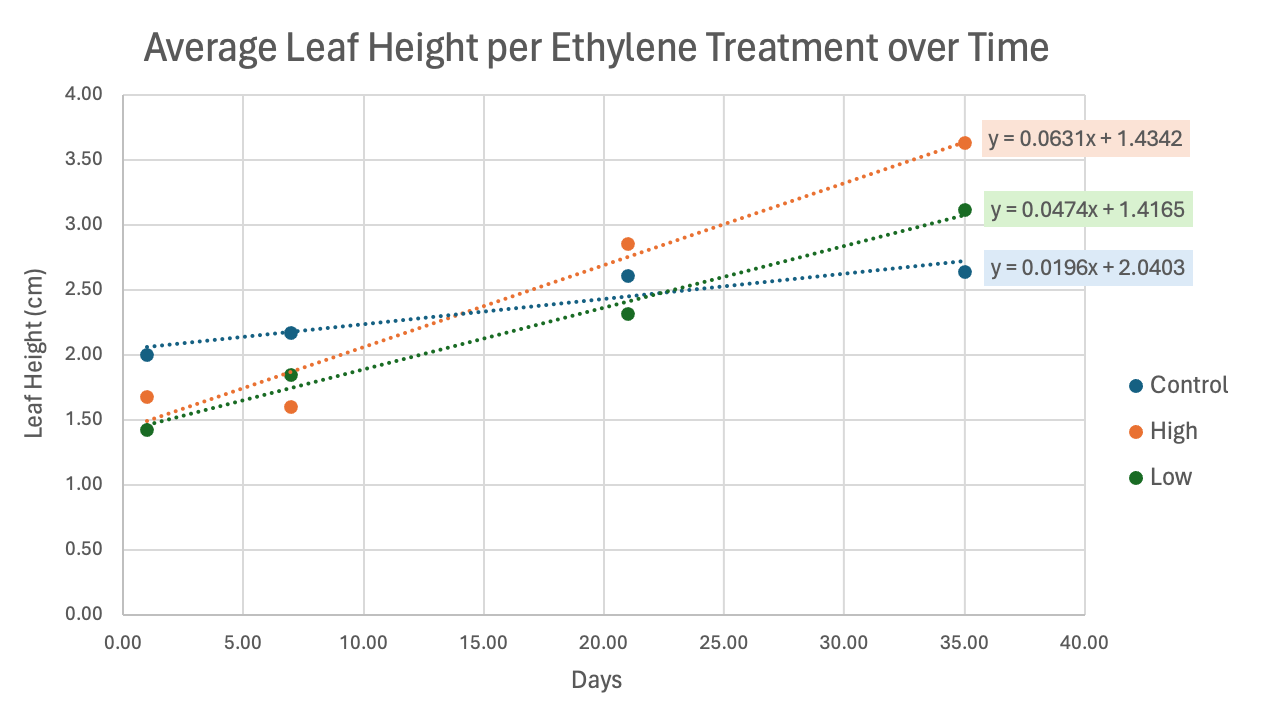
\includegraphics[width=\linewidth]{graph1.png}
    \captionof{figure}{Average leaf height per ethylene treatment in \textit{Narcissus spp.} vegetation over time.}
  \end{minifig}

  \textbf{Discussion}\\
  Increasing ethylene exposure did not exhibit significant negative impact on final leaf height; no clear trend was observed (R\textsuperscript{2} = 0.0035; Figure 1). In fact, the regression slope was slightly positive, indicating a slight increase in leaf height with increasing ethylene concentration. This is corroborated by data from Figure 2, which showed that ethylene-treated plants grew faster and had a higher final leaf height on average than control. While these findings initially suggest that ethylene may have a positive effect on plant growth, it is more likely that the results are due to limitations. Future research should focus on increasing the amount of data collected, i.e. frequency, duration, different ethylene concentrations. If the plants were not exposed to \textit{enough} ethylene for a sufficient \textit{duration}, the phenomenon may not have been observed.
  
\end{multicols}

\clearpage

\setstretch{1.5}

\printbibliography

\end{document}